\chapter{Sample Covariance Matrix}

Suppose $\left\{\bfx\right\}$ be a sequence of random vectors defined in $\bbR^{n}$, and $\left(x_{i}\right)_{1\leq i\leq n}$ be the components of the random vector $\bfx$, such that
\begin{equation*}
	E\left(\bfx\right)=0,\quad E\left(\bfx\otimes\bfx\right)=\mathbf{I}_{n}
\end{equation*}
where $\bfx$ is also called \textbf{isotropic} random vector.

Suppose $\left\{m_{n}\right\}$ be a sequence defined in $\mathbb{N}$ such that
\begin{equation*}
	0<\underline{\rho}:=\liminf_{n\rightarrow\infty}\frac{n}{m_{n}}\leq\limsup_{n\rightarrow\infty}\frac{n}{m_{n}}=:\bar{\rho}<\infty
\end{equation*}

Let $\bfx_{1},\ldots,\bfx_{m_{n}}$ be iid copies of $\bfx$, and $\mathbb{X}$ be the $m_{n}\times n$ random matrix with iid rows $\bfx_{1},\ldots,\bfx_{m_{n}}$, and their empirical covariance matrix is
\begin{equation*}
	\widehat{\bfSigma}:=\frac{1}{m_{n}}\sum_{i=1}^{m_{n}}\bfx_{i}\otimes\bfx_{i}=\frac{1}{m_{n}}\mathbb{X}^{\prime}\mathbb{X}
\end{equation*}
which is a $n\times n$ symmetric positive semidefinite random matrix, and
\begin{equation*}
	E\left(\widehat{\bfSigma}\right)=\bbE\left(\bfx\otimes\bfx\right)=\mathbf{I}_{n}
\end{equation*}

For convenience, we define the random matrix
\begin{equation*}
	\bfA:=m_{n}\widehat{\bfSigma}=\mathbb{X}^{\prime}\mathbb{X}=\sum_{i=1}^{m_{n}}\bfx_{i}\otimes\bfx_{i}
\end{equation*}

\section{Eigenvalues and Singular Values}

\begin{theorem}
	The eigenvalues of $\bfA$ are squares of the singular values of $\mathbb{X}$, in particularly
	\begin{equation*}
		\lambda_{\max}\left(\bfA\right)=s_{\max}\left(\mathbb{X}\right)^{2}=\max_{\|\bfx\|=1}\left\|\mathbb{X}\bfx\right\|^{2}=\left\|\mathbb{X}\right\|_{2}^{2}
	\end{equation*}
	if $m_{n}\geq n$, then
	\begin{equation*}
		\lambda_{\min}\left(\bfA\right)=s_{\min}\left(\mathbb{X}\right)^{2}=\min_{\|\bfx\|=1}\left\|\mathbb{X}\bfx\right\|^{2}=\left\|\mathbb{X}^{-1}\right\|_{2}^{-2}
	\end{equation*}
\end{theorem}

\begin{proof}

\end{proof}

\section{Laguerre Orthogonal Ensemble}

\begin{definition}[Wishart Distribution]
	Suppose $\mathbb{X}$ be a $p\times n$ matrix, each column of which is independently drawn from a $p$-variate normal distribution with zero means:
	\begin{equation*}
		\bfx_{i}=\left(x_{i}^{1},\ldots,x_{i}^{p}\right)^{\prime}\sim N_{p}(0,\bfSigma)
	\end{equation*}
	Then the Wishart distribution is the probability distribution of the $p\times p$ random matrix,
	\begin{equation}
		\bfM=\mathbb{X}^{\prime}\mathbb{X}=\sum_{i=1}^{n}\bfx_{i}\bfx_{i}^{\top}
	\end{equation}
	and which can be denoted by
	\begin{equation*}
		\bfM\sim W_{p}\left(\bfSigma,n\right)
	\end{equation*}
	If $p=\bfSigma=1$, then this distribution is a chi-squared distribution with $n$ degrees of freedom.
\end{definition}

\begin{theorem}
	If $n\geq p$, the probability density function of $\bfM$ is
	\begin{equation}
		f\left(\bfM\right)=\frac{1}{2^{np/2}\left[\operatorname{det}\left(\bfSigma\right)\right]^{n/2}\Gamma_{p}\left(\frac{n}{2}\right)}\operatorname{det}\left(\bfM\right)^{(n-p-1)/2}\exp\left[-\frac{1}{2}\operatorname{tr}\left(\bfSigma^{-1}\bfM\right)\right]
		\label{eq:pdf-wishart}
	\end{equation}
	concerning the Lebesque measure on the cone of symmetric positive definite matrices. Here, $\Gamma_{p}$ is the multivariate gamma function defined as
	\begin{equation*}
		\Gamma_{p}\left(\frac{n}{2}\right)=\pi^{p(p-1)/4}\prod_{j=1}^{p}\Gamma\left(\frac{n}{2}-\frac{j-1}{2}\right)
	\end{equation*}
\end{theorem}

\begin{remark}
	Especially, if the random variables $\left(x_{i}\right)_{1\leq i\leq n}$ are iid standard Gaussians, then the distribution of the random matrix $\widehat{\bfSigma}$ can be derived from the Wishart distribution. The probability density function of $\widehat{\bfSigma}$ can be derived from \eqref{eq:pdf-wishart}, since
	\begin{equation*}
		\bfA\sim W_{n}\left(\mathbf{I}_{n},m_{n}\right),\quad\operatorname{det}\left(\widehat{\bfSigma}\right)=m_{n}^{-n}\operatorname{det}\left(\bfA\right),\quad\operatorname{tr}\left(\widehat{\bfSigma}\right)=m_{n}^{-1}\operatorname{tr}\left(\bfA\right)
	\end{equation*}
	thus,
	\begin{equation}
		f\left(\widehat{\bfSigma}\right)=\frac{m_{n}^{-n(m_{n}-n-1)/2+1}}{2^{m_{n}n/2}\Gamma_{n}\left(\frac{m_{n}}{2}\right)}\operatorname{det}\left(\widehat{\bfSigma}\right)^{(m_{n}-n-1)/2}\exp\left[-\frac{m_{n}}{2}\operatorname{tr}\left(\widehat{\bfSigma}\right)\right]
	\end{equation}
\end{remark}

\begin{theorem}
	If the random variables $\left(x_{i}\right)_{1\leq i\leq n}$ are iid standard Gaussians, the joint probability density function of eigenvalues of $\widehat{\bfSigma}$ is
	\begin{equation}
		p\left(\bfLambda\right)=\widetilde{Q}_{m_{n},n}^{-1}\exp\left(-\frac{m_{n}}{2}\sum_{k=1}^{n}\lambda_{k}\right)\prod_{k=1}^{n}\lambda_{k}^{(m_{n}-n-1)/2}\prod_{i<j}\left|\lambda_{i}-\lambda_{j}\right|
		\label{eq:jpdf-eigenvalues-sigma}
	\end{equation}
	where
	\begin{equation*}
		0\leq\lambda_{1}\leq\ldots\leq\lambda_{n}<\infty
	\end{equation*}
	and $\widetilde{Q}_{m_{n},n}$ is the normalization constant.
\end{theorem}

\begin{proof}
	Fisrt, we will give the characteristic function of $\widehat{\bfSigma}$, i.e.,
	\begin{equation*}
		\varphi_{\widehat{\bfSigma}}\left(\mathbf{P}\right)=E\left[\exp\left(\imath\sum_{1\leq i\leq j\leq n}P_{ij}\widehat{\bfSigma}_{ji}\right)\right]=E\left[\exp\left(\imath\operatorname{tr}\left(\mathbf{P}\widehat{\bfSigma}\right)\right)\right]
	\end{equation*}
	where $\left\{P_{ij}\right\}_{1\leq i\leq j\leq n}\in\bbR^{(n+1)n/2}$ and $\mathbf{P}$ is a real symmetric matrix, that
	\begin{equation*}
		\mathbf{P}=\left\{\widehat{P}_{ij},\widehat{P}_{ij}=\widehat{P}_{ji}\right\}_{i,j=1}^{n},\quad\widehat{P}_{ij}=\begin{cases}P_{ii}, & i=j \\ P_{ij} / 2, & i<j \end{cases}
	\end{equation*}
	Thus, we have
	\begin{equation*}
		\begin{aligned}
			= & \int_{\bbR^{m_{n}\times n}}\exp\left(\imath\operatorname{tr}\left(\mathbf{P}\widehat{\bfSigma}\right)\right)\cdot(2\pi)^{-m_{n}n/2}\exp\left(-\frac{1}{2}\sum_{k=1}^{m_{n}}\sum_{i=1}^{n}\left(x_{i}^{(k)}\right)^{2}\right)\prod_{k=1}^{m_{n}}\prod_{i=1}^{n}\dif x_{i}^{(k)} \\
			= & \int_{\bbR^{m_{n}\times n}}(2\pi)^{-m_{n}n/2}\exp\left(-\frac{1}{2}\sum_{k=1}^{m_{n}}\sum_{i=1}^{n}\sum_{j=1}^{n}\bfQ_{ij}x_{i}^{(k)}x_{j}^{(k)}\right)\prod_{k=1}^{m_{n}}\prod_{i=1}^{n}\dif x_{i}^{(k)}
		\end{aligned}
	\end{equation*}
	where
	\begin{equation*}
		\bfQ=\mathbf{I}_{n}-\frac{2\imath}{m_{n}}\mathbf{P}
	\end{equation*}
	Since $\left(x_{i}^{(k)}\right)_{1\leq i\leq n}$ are iid standard Gaussians,
	\begin{equation*}
		\begin{aligned}
			= & \left[\int_{\bbR^{n}}(2\pi)^{-n/2}\exp\left(-\frac{1}{2}\sum_{i=1}^{n}\sum_{j=1}^{n}\bfQ_{ij}x_{i}x_{j}\right)\prod_{i=1}^{n}\dif x_{i}\right]^{m_{n}}                                                                                    \\
			= & \left[\int_{\bbR^{n}}(2\pi)^{-n/2}\exp\left(-\frac{1}{2}\bfx^{\top}\bfQ\bfx\right)\dif\bfx\right]^{m_{n}}                                                                                                                                 \\
			= & \left[\operatorname{det}\left(\bfQ\right)^{-\frac{1}{2}}\int_{\bbR^{n}}(2\pi)^{-n/2}\exp\left(-\frac{1}{2}\left(\bfQ^{\frac{1}{2}}\bfx\right)^{\prime}\left(\bfQ^{\frac{1}{2}}\bfx\right)\right)\dif\bfQ^{\frac{1}{2}}\bfx\right]^{m_{n}} \\
			= & \left[\operatorname{det}\left(\bfQ\right)\right]^{-m_{n}/2}
		\end{aligned}
	\end{equation*}
	thus,
	\begin{equation}
		\left[\operatorname{det}\left(\bfQ\right)\right]^{-m_{n}/2}=\left[\operatorname{det}\left(\mathbf{I}_{n}-\frac{2\imath}{m_{n}}\mathbf{P}\right)\right]^{-m_{n}/2}=\prod_{k=1}^{n}\left(1-\frac{2\imath}{m_n}p_{k}\right)^{-m_{n}/2}
		\label{eq:characteristic-function-wishart-result-1}
	\end{equation}
	where $\{p_{k}\}_{k=1}^{n}$ are the eigenvalues of $\mathbf{P}$.

	Then, we will show that the characteristic function of (\ref{eq:jpdf-eigenvalues-sigma}) coincides with the above function. By the Wishart distribution, the probability density of the real symmetric and positive definite random matrix $\widehat{\bfSigma}$ is
	\begin{equation}
		\widetilde{Q}_{m_{n},n}^{-1}\exp\left[-\frac{m_{n}}{2}\operatorname{tr}\left(\widehat{\bfSigma}\right)\right]\left[\operatorname{det}\left(\widehat{\bfSigma}\right)\right]^{(m_{n}-n-1)/2}\dif\widehat{\bfSigma}
		\label{eq:wishart-distribution-sigma}
	\end{equation}
	where $\widetilde{Q}_{m_{n},n}$ is the normalization constant. Then, the characteristic function of (\ref{eq:wishart-distribution-sigma}), i.e.,
	\begin{equation*}
		\widetilde{Q}_{m_{n},n}^{-1}\int_{\mathcal{S}_{n}^{+}}\exp\left[\imath\operatorname{tr}\left(\mathbf{P}\widehat{\bfSigma}\right)-\frac{m_{n}}{2}\operatorname{tr}\left(\widehat{\bfSigma}\right)\right]\left[\operatorname{det}\left(\widehat{\bfSigma}\right)\right]^{(m_{n}-n-1)/2}\dif\widehat{\bfSigma}
	\end{equation*}
	where the integration is over the set $\mathcal{S}_{n}^{+}$ of $n\times n$ real symmetric and positive definite matrices. Since
	\begin{equation*}
		\sum_{k=1}^{n}\lambda_{k}=\operatorname{tr}\left(\widehat{\bfSigma}\right),\quad\prod_{k=1}^{n}\lambda_{k}^{(m_{n}-n-1)/2}=\left[\operatorname{det}\left(\widehat{\bfSigma}\right)\right]^{(m_{n}-n-1)/2}
	\end{equation*}
	and
	\begin{equation*}
		\dif\widehat{\bfSigma}=\prod_{i<j}\left|\lambda_{i}-\lambda_{j}\right|\dif\bfLambda H_{1}\left(\dif O\right)
	\end{equation*}
	where $H_{1}$ is the normalized Haar measure of $O(n)$, and the integration over $\bfLambda$ and $O\in O(n)$ are independent. Since the orthogonal invariance of the density of (\ref{eq:wishart-distribution-sigma}), and the characteristic function is
	\begin{equation}
		Q_{m_{n},n}^{-1}\int_{\left(\bbR_{+}\right)^{n}}\exp\left[\sum_{k=1}^{n}\left(\imath p_{k}-\frac{m_{n}}{2}\right)\lambda_{k}\right]\prod_{k=1}^{n}\lambda_{k}^{(m_{n}-n-1)/2}\prod_{i<j}\left|\lambda_{i}-\lambda_{j}\right|\dif\bfLambda
		\label{eq:characteristic-function-wishart}
	\end{equation}
	where $Q_{m_{n},n}=m_{n}!\widetilde{Q}_{m_{n},n}$.

	If we viewed (\ref{eq:characteristic-function-wishart-result-1}) and (\ref{eq:characteristic-function-wishart}) as the function of $\{p_{k}\}_{k=1}^{n}\in\bbR^{n}$, then they can be \textbf{analytic continuation} to the domain
	\begin{equation*}
		\left\{p_{k}+\imath p_{k}^{\prime},p_{k}^{\prime}\geq 0\right\}_{k=1}^{n}
	\end{equation*}
	If we replace $\left\{p_{k}\right\}_{k=1}^{n}$ by $\left\{\imath p_{k}^{\prime},p_{k}^{\prime}\geq 0\right\}_{k=1}^{n}$ on \eqref{eq:characteristic-function-wishart-result-1} since this is a set of the uniqueness of both (\ref{eq:characteristic-function-wishart-result-1}) and eqref{eq:characteristic-function-wishart} analytic functions, we have
	\begin{equation*}
		Q_{m_{n},n}^{-1}\int_{\left(\bbR_{+}\right)^{n}}\exp\left[-\frac{m_{n}}{2}\sum_{k=1}^{n}q_{k}\lambda_{k}\right]\prod_{k=1}^{n}\lambda_{k}^{(m_{n}-n-1)/2}\prod_{i<j}\left|\lambda_{i}-\lambda_{j}\right|\dif\bfLambda
	\end{equation*}
	where $q_{k}=1+\frac{2p_{k}^{\prime}}{m_{n}}\geq 1,k=1,\ldots,n$, and since
	\begin{equation*}
		\forall i,j\quad\frac{q_{i}}{q_{j}}=\frac{1+\frac{2p_{i}^{\prime}}{m_{n}}}{1+\frac{2p_{j}^{\prime}}{m_{n}}}\rightarrow 1,\ \text{as}\ \quad m_{n}\rightarrow\infty
	\end{equation*}
	we have
	\begin{equation*}
		\prod_{i<j}\left|q_{i}\lambda_{i}-q_{j}\lambda_{j}\right|=\prod_{i<j}q_{i}\left|\lambda_{i}-\frac{q_{j}}{q_{i}}\lambda_{j}\right|\rightarrow\prod_{k=1}^{n}q_{k}^{(n-1)/2}\prod_{i<j}\left|\lambda_{i}-\lambda_{j}\right|,\ \text{as}\ \quad m_{n}\rightarrow\infty
	\end{equation*}
	thus,
	\begin{equation*}
		\begin{array}{c}
			\prod_{k=1}^{n}q_{k}^{-m_{n}/2}\cdot Q_{m_{n},n}^{-1}\int_{\left(\bbR_{+}\right)^{n}}\exp\left[-\frac{m_{n}}{2}\sum_{k=1}^{n}q_{k}\lambda_{k}\right]\prod_{k=1}^{n}\left(q_{k}\lambda_{k}\right)^{(m_{n}-n-1)/2}\cdot \\
			\prod_{i<j}\left|q_{i}\lambda_{i}-q_{j}\lambda_{j}\right|\dif\bfq\bfLambda
		\end{array}
	\end{equation*}
	Since
	\begin{equation*}
		\forall k\quad q_{k}\lambda_{k}\rightarrow\lambda_{k},\ \text{as}\ \quad m_{n}\rightarrow\infty
	\end{equation*}
	we can "lifting" from $\left\{\lambda_{k}\right\}_{k=1}^{n}$ to $\mathcal{S}_{n}^{+}$ bring the integral to
	\begin{equation*}
		\prod_{k=1}^{n}\left(1+\frac{2p_{k}^{\prime}}{m_{n}}\right)^{-m_{n}/2}\widetilde{Q}_{n}^{-1}\int_{\mathcal{S}_{n}^{+}}\exp\left[-\frac{m_{n}}{2}\operatorname{tr}\left(\widehat{\bfSigma}\right)\right]\left[\operatorname{det}\left(\widehat{\bfSigma}\right)\right]^{(m_{n}-n-1)/2}\dif\widehat{\bfSigma}
	\end{equation*}
	The integral here is equal to $\widetilde{Q}_{n}$, the normalization constant of the probability measure (\ref{eq:wishart-distribution-sigma}). If we replace $\left\{\imath p_{k}^{\prime}\right\}_{k=1}^{n}$ back by $\left\{p_{k}\right\}_{k=1}^{n}$, then the above expression is
	\begin{equation*}
		\prod_{k=1}^{n}\left(1-\frac{2\imath}{m_n}p_{k}\right)^{-m_{n}/2}
	\end{equation*}
	which coincides with (\ref{eq:characteristic-function-wishart-result-1}). Thus the probability law of the Wishart matrices of $\bfSigma$ given by (\ref{eq:wishart-distribution-sigma}) implies that the corresponding joint probability density of eigenvalues is given by (\ref{eq:jpdf-eigenvalues-sigma}) for $\bfSigma$.
\end{proof}

\begin{definition}[Laguerre Orthogonal Ensemble]
	For the $n\times n$ Laguerre orthogonal ensembles of statistics, the joint probability density function of eigenvalues is
	for arbitrary parameter $\beta>0$ and $\alpha>-\frac{2}{\beta}$, is
	\begin{equation}
		p\left(\bfLambda\right)=K_{\alpha,\beta}\exp\left(-\frac{\beta}{2}\sum_{k=1}^{n}\lambda_{k}\right)\prod_{k=1}^{n} \lambda_{k}^{\frac{\alpha\beta}{2}}\prod_{i<j}\left|\lambda_{i}-\lambda_{j}\right|^{\beta}
		\label{eq:laguerre-orthogonal-ensemble}
	\end{equation}
	where
	\begin{equation*}
		0\leq\lambda_{1}\leq\ldots\leq\lambda_{n}<\infty
	\end{equation*}
	and $K_{n,m}$ are normalization constant.
\end{definition}

And Equation (\ref{eq:laguerre-orthogonal-ensemble}) can be written in the standard Boltzmann-Gibbs form, that,
\begin{equation*}
	p\left(\bfLambda\right)\propto\exp\left[-\beta E\left(\bfLambda\right)\right]
\end{equation*}
where
\begin{equation}
	E\left(\bfLambda\right)=\frac{1}{2}\sum_{k=1}^{n}\left(\lambda_{k}-\alpha\log\lambda_{k}\right)-\frac{1}{2}\sum_{i\neq j}\left|\lambda_{i}-\lambda_{j}\right|
\end{equation}

\begin{remark}
	For the (\ref{eq:jpdf-eigenvalues-sigma}), which can be written as (\ref{eq:laguerre-orthogonal-ensemble}) form, that,
	\begin{equation*}
		p\left(\bfLambda\right)\propto\exp\left[-\beta m_{n}E\left(\bfLambda\right)\right]
	\end{equation*}
	where $\beta=1$ and
	\begin{equation*}
		E\left(\bfLambda\right)=\frac{m_{n}}{2}\sum_{k=1}^{n}\left[\lambda_{k}-\left(\frac{m_{n}-n-1}{m_{n}}\right)\log\lambda_{k}\right]-\frac{1}{2m_{n}}\sum_{i\neq j}\left|\lambda_{i}-\lambda_{j}\right|
	\end{equation*}
\end{remark}

\section{Mar\v{c}enko-Pastur Theorem}

In this section, we will investigate the empirical spectral measure of $\widehat{\bfSigma}$, which converges to a nonrandom distribution --- Mar\v{c}enko-Pastur distribution. Before further proof, we will introduce some basic concepts and tools.

With the above tools, we can prove the Mar\v{c}enko-Pastur Theorem. Here, we only suppose $\bfx$ has some smooth tail condition.
\begin{theorem}[Mar\v{c}enko-Pastur Theorem] \label{thm:marcenko-pastur-theorem}
	Consider the resolvent
	\begin{equation*}
		\bfQ(z)=\left(\widehat{\bfSigma}-z\mathbf{I}_{n}\right)^{-1}
	\end{equation*}
	Then, if
	\begin{equation*}
		\frac{n}{m_{n}}\rightarrow\rho\ \text{with}\ \rho\in(0,\infty),\ \text{as}\ n\rightarrow\infty
	\end{equation*}
	we have
	\begin{equation*}
		\bfQ(z)\leftrightarrow\overline{\bfQ}(z),\quad\overline{\bfQ}(z)=m(z)\mathbf{I}_{n}
	\end{equation*}
	with $(z,m(z))$ the unique solution in $\mathcal{Z}\left(\mathbb{C}\backslash\left[(1-\sqrt{\rho})^{2},(1+\sqrt{\rho})^{2}\right]\right)$ be
	\begin{equation*}
		zcm^{2}(z)-(1-c-z)m(z)+1=0
	\end{equation*}
	where the function $m(z)$ is the Stieltjes transform of the probability measure $\mu$ given explicitly by
	\begin{equation*}
		\mu(\dif x)=\left(1-\rho^{-1}\right)^{+}\delta_{0}(x)+\frac{\sqrt{\left(x-a_{-}\right)^{+}\left(a_{+}-x\right)^{+}}}{2\pi\rho x}\dif x
	\end{equation*}
	where $a_{\pm}=(1 \pm \sqrt{\rho})^{2}$ and $(x)^{+}=\max (0, x)$, and is known as the Mar\v{c}enko-Pastur distribution. In particular, with probability one, the empirical spectral measure $\mu_{\widehat{\bfSigma}}$ converges weakly to $\mu $.
\end{theorem}

\begin{figure}[htbp]
	\centering
	\begin{subfigure}{.45\linewidth}
		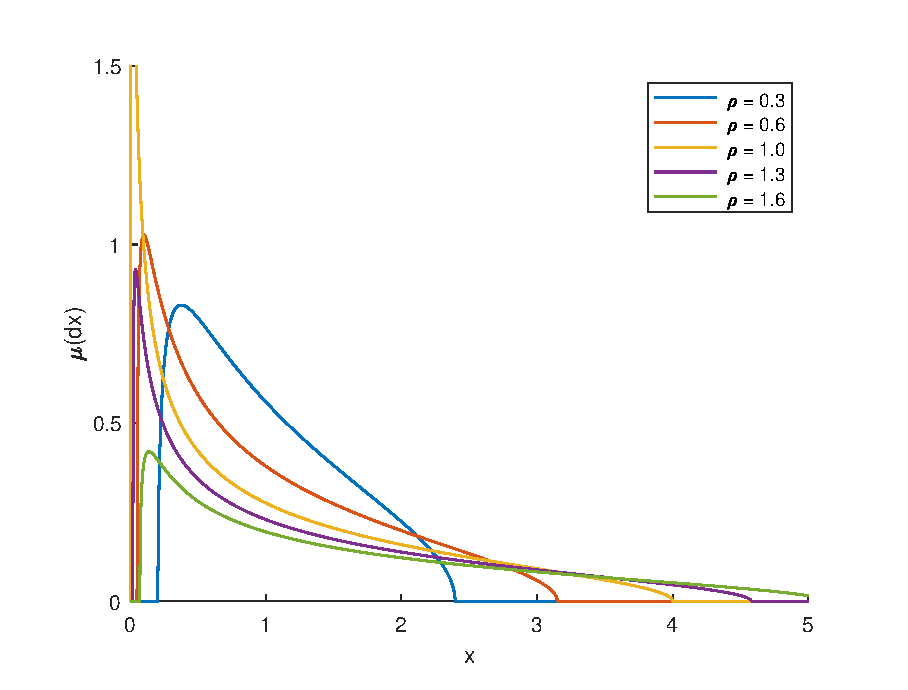
\includegraphics[width=\textwidth]{random-matrix-theory/figures/marchenko-pastur-distribution.eps}
		\caption{The Mar\v{c}enko-Pastur Distribution for $\rho=0.3,0.6,1,1.3,1.6$}
	\end{subfigure}
	\begin{subfigure}{.45\linewidth}
		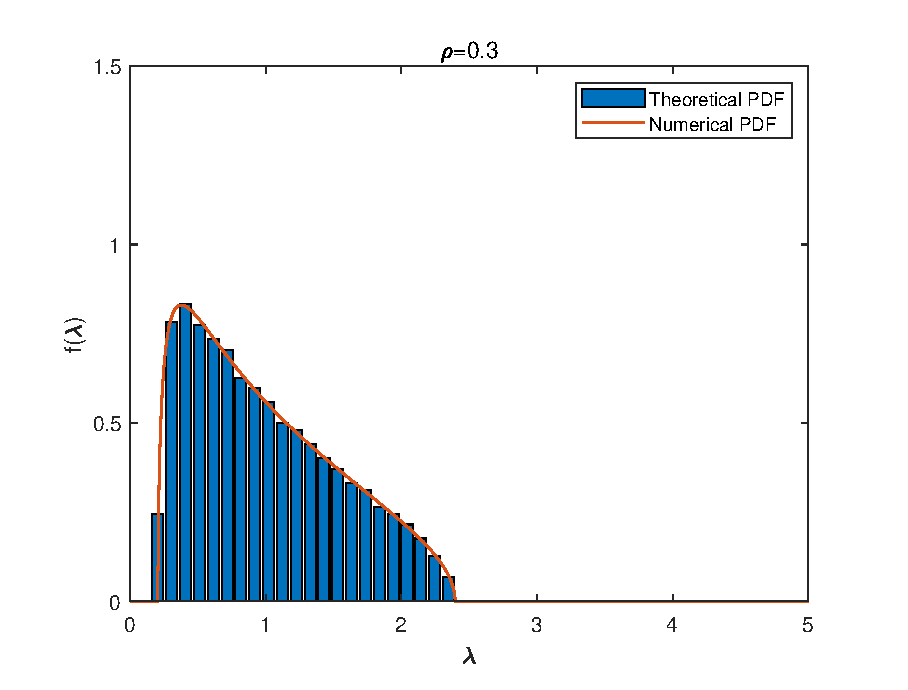
\includegraphics[width=\textwidth]{random-matrix-theory/figures/marchenko-pastur-theorem-simulation.eps}
		\caption{Simulation Results of the Mar\v{c}enko-Pastur Theorem When $\rho=0.3$}
	\end{subfigure}
	\caption{Illustrations of the Mar\v{c}enko-Pastur Theorem}
\end{figure}

\begin{proof}
	(Intuitive Proof) Suppose $\overline{\bfQ}(z)=\bfF(z)^{-1}$ for some matrix $\bfF(z)$. To prove $\overline{\bfQ}(z)$ to be a deterministic equivalent for $\bfQ(z)$, particularly,
	\begin{equation*}
		\frac{1}{n}\operatorname{tr}\bfA(\bfQ(z)-\overline{\bfQ}(z))\rightarrow 0\quad\text{a.s.}
	\end{equation*}
	where $\bfA$ is arbitrary, deterministic, and such that $\|\bfA\|=1$. By Lemma~\ref{lem:resolvent-identity}, we have
	\begin{equation*}
		\begin{aligned}
			\bfQ(z)-\overline{\bfQ}(z)= & \bfQ(z)\left(\bfF(z)+z\mathbf{I}_{n}-\widehat{\bfSigma}\right) \overline{\bfQ}(z)                                      \\
			=                           & \bfQ(z)\left(\bfF(z)+z\mathbf{I}_{n}-\frac{1}{m_{n}}\sum_{i=1}^{m_{n}}\bfx_{i}\bfx_{i}^{\top}\right)\overline{\bfQ}(z)
		\end{aligned}
	\end{equation*}
	Thus, we turn to prove that,
	\begin{equation*}
		\frac{1}{n}\operatorname{tr}\left[\left(\bfF(z)+z\mathbf{I}_{n}\right)\overline{\bfQ}(z)\bfA\bfQ(z)\right]-\frac{1}{n}\cdot\frac{1}{m_{n}}\sum_{i=1}^{m_{n}}\bfx_{i}^{\top}\overline{\bfQ}(z)\bfA\bfQ(z)\bfx_{i}\rightarrow 0\quad\text{a.s.}
	\end{equation*}
	By Lemma~\ref{lem:sherman-morrison}, we have
	\begin{equation*}
		\bfQ(z)\bfx_{i}=\frac{\bfQ_{-i}(z)\bfx_{i}}{1+\frac{1}{m_{n}}\bfx_{i}^{\top}\bfQ_{-i}(z)\bfx_{i}}
	\end{equation*}
	where
	\begin{equation*}
		\bfQ_{-i}(z)=\left(\frac{1}{m_{n}}\sum_{j\neq i}\bfx_{j}\bfx_{j}^{\prime}-z\mathbf{I}_{n}\right)^{-1}
	\end{equation*}
	is independent of $\bfx_{i}$. By Lemma~\ref{lem:quadratic-form-close-to-the-trace}, we have
	\begin{equation*}
		\frac{1}{n}\bfx_{i}^{\top}\overline{\bfQ}(z)\bfA\bfQ(z)\bfx_{i}=\frac{\frac{1}{n}\bfx_{i}^{\top}\overline{\bfQ}(z)\bfA\bfQ_{-i}(z)\bfx_{i}}{1+\frac{1}{m_{n}}\bfx_{i}^{\top}\bfQ_{-i}(z)\bfx_{i}}\simeq\frac{\frac{1}{n}\operatorname{tr}\left[\overline{\bfQ}(z)\bfA\bfQ_{-i}(z)\right]}{1+\frac{1}{m_{n}}\operatorname{tr}\left[\bfQ_{-i}(z)\right]}
	\end{equation*}
	Hence, we need to prove the approximation that
	\begin{equation*}
		\frac{1}{n}\operatorname{tr}\left[\left(\bfF(z)+z\mathbf{I}_{n}\right)\overline{\bfQ}(z)\bfA\bfQ(z)\right]\simeq\frac{\frac{1}{n}\operatorname{tr}\left[\overline{\bfQ}(z)\bfA\bfQ(z)\right]}{1+\frac{1}{m_{n}}\operatorname{tr}\left[\bfQ(z)\right]}
	\end{equation*}
	If $\bfF(z)$ exist, for the approximation above to hold, $\bfF(z)$ must be of the type
	\begin{equation*}
		\bfF(z)\simeq\left(-z+\frac{1}{1+\frac{1}{m_{n}}\operatorname{tr}\bfQ(z)}\right)\mathbf{I}_{n}
	\end{equation*}
	By Equation~\ref{eq:relation-between-empirical-spectral-measures-stieltjes-transform-and-its-resolvent}, we have,
	\begin{equation*}
		m(z)\equiv\frac{1}{n}\operatorname{tr}\left[\overline{\bfQ}(z)\right]=\frac{1}{n}\operatorname{tr}\left[\bfF(z)^{-1}\right]
	\end{equation*}
	taking $\bfA=\mathbf{I}_{n}$, we have
	\begin{equation*}
		\frac{1}{n}\operatorname{tr}\left[\bfQ(z)\right]\simeq\frac{1}{n}\operatorname{tr}\left[\overline{\bfQ}(z)\right]=m(z)=\frac{1}{-z+\frac{1}{1+\frac{n}{m_{n}}\frac{1}{n}\operatorname{tr}\left[\bfQ(z)\right]}}\simeq\frac{1}{-z+\frac{1}{1+\rho m(z)}}
	\end{equation*}
	As $n,m_{n}\rightarrow\infty$, $m(z)$ is solution to
	\begin{equation*}
		m(z)=\frac{1}{-z+\frac{1}{1+\rho m(z)}}
	\end{equation*}
	or equivalently
	\begin{equation*}
		z\rho m^{2}(z)-(1-\rho-z)m(z)+1=0
	\end{equation*}
	This equation has two solutions defined via the two values of the complex square root function. Let
	\begin{equation*}
		z=r\mathrm{e}^{\imath\theta}\ \text{where}\ r\geq 0,\theta\in[0,2\pi)\Rightarrow\sqrt{z}\in\left\{\pm\sqrt{r}\mathrm{e}^{\imath\theta/2}\right\}
	\end{equation*}
	and we can conclude that
	\begin{equation*}
		m(z)=\frac{1-\rho-z}{2\rho z}+\frac{\sqrt{\left((1+\sqrt{\rho})^{2}-z\right)\left((1-\sqrt{\rho})^{2}-z\right)}}{2\rho z}
	\end{equation*}
	only one of which is such that $\Im[z]\Im[m(z)]>0$ as imposed by the definition of Stieltjes transforms. By the inverse Stieltjes transform theorem, Theorem~\ref{thm:inverse-stieltjes-transform}, we find that $m(z)$ is the Stieltjes transform of the measure $\mu$ with
	\begin{equation*}
		\mu([a,b])=\frac{1}{\pi}\lim_{\epsilon\downarrow 0}\int_{a}^{b}\Im[m(x+\imath\epsilon)]\dif x
	\end{equation*}
	for all continuity points $a,b\in\bbR$ of $\mu$. This term under the square root in $m(z)$ is negative only in the set
	\begin{equation*}
		\left[(1-\sqrt{\rho})^{2},(1+\sqrt{\rho})^{2}\right]
	\end{equation*}
	(and thus of non-real square root), the latter defines the support of the continuous part of the measure $\mu$ with density
	\begin{equation*}
		\frac{\sqrt{\left((1+\sqrt{\rho})^{2}-x\right)\left(x-(1-\sqrt{\rho})^{2}\right)}}{2\rho\pi x}
	\end{equation*}
	at point $x$ in the set. The case $x=0$ brings a discontinuity in $\mu$ with weight equal to
	\begin{equation*}
		\mu(\{0\})=-\lim_{y\downarrow 0}\imath ym(\imath y)=\frac{\rho-1}{2\rho}\pm\frac{\rho-1}{2\rho}
	\end{equation*}
	where the sign is established by a second order development of $z m(z)$ in the neighborhood of zero: that is, "+" for $c>1$ inducing a mass $1-1/\rho$ for $p>n$, or "-" for $c<1$ in which case $\mu(\{0\})=0$ and $\mu$ has no mass at zero.
\end{proof}

\begin{remark}
	The asymptotic phenomenon holds not only in the Gaussian case, which also holds
	\begin{enumerate}
		\item if $\left(x_{i}\right)_{1\leq i\leq n}$ are iid with finite second moment.
		\item if $\bfx$ is isotropic and log-concave\footnote{A probability measure $\mu$ on $\bbR^{n}$ with density $\varphi$ is log-concave when $\varphi=e^{-V}$ with $V$ convex.} random vector.
	\end{enumerate}
\end{remark}

\section{Limits of Extreme Eigenvalues}

The weak convergence in Theorem~\ref{thm:marcenko-pastur-theorem} does not provide much information at the edge on the behavior of the extremal atoms, and what one can extract is that
\begin{equation}
	\limsup_{n\rightarrow\infty}\lambda_{\min}\left(\widehat{\bfSigma}\right)\leq(1-\sqrt{\rho})^{2}\leq(1+\sqrt{\rho})^{2}\leq\liminf_{n\rightarrow\infty}\lambda_{\max}\left(\widehat{\bfSigma}\right)\quad\text{a.s.}
\end{equation}
where the first inequality is considered only in the case where $m_{n}\geq n$.

The weak convergence above does not provide much information at the edge on the behavior of the extremal atoms. Now, we have more exact result, that if $\left(X_{n,k}\right)_{n\geq 1,1\leq k\leq n}$ are iid with finite fourth moment then,
\begin{equation} \label{eq:limits-of-extreme-eigenvalues-of-sample-covariance-matrices}
	(1-\sqrt{\rho})^{2}=\lim_{n\rightarrow\infty}\lambda_{\min}\left(\widehat{\bfSigma}\right)\leq\lim_{n\rightarrow\infty}\lambda_{\max}\left(\widehat{\bfSigma}\right)=(1+\sqrt{\rho})^{2}\quad\text{a.s.}
\end{equation}
where the first inequality is considered only in the case where $m_{n}\geq n$.

\begin{remark}
	The convergence of the smallest eigenvalue in the left-hand side of (\ref{eq:limits-of-extreme-eigenvalues-of-sample-covariance-matrices}) holds if $\left(x_{i}\right)_{1\leq i\leq n}$ are iid with finite second moment.
\end{remark}

\begin{theorem}
	If $\bar{\rho}<1$ (in particular $m_{n}>n$ for $n\gg 1$ ) and if the centered isotropic random vector $\bfx$ is log-concave or if $\left(x_{i}\right)_{1\leq i\leq n}$ are iid then
	\begin{equation}
		\liminf_{n\rightarrow\infty}\frac{E\left(\lambda_{\min}\left(\bfA_{n}\right)\right)}{\left(\sqrt{m_{n}}-\sqrt{n}\right)^{2}}\geq 1
	\end{equation}
	If additionally $\lim_{n\rightarrow\infty}\frac{n}{m_{n}}=\rho$ with $\rho \in(0,1)$, in other words $\underline{\rho}=\bar{\rho}\in(0,1)$, then
	\begin{equation}
		\lambda_{\min}\left(\widehat{\bfSigma}_{n}\right)\stackrel{p}{\longrightarrow}(1-\sqrt{\rho})^{2}\ \text{as}\ n\rightarrow\infty
	\end{equation}
\end{theorem}

\begin{proof}

\end{proof}

\begin{theorem}
	If the centered isotropic random vector $\bfx$ is log-concave or if $\left(x_{i}\right)_{1\leq i\leq n}$ are iid with finite 4-th moment then
	\begin{equation}
		\limsup_{n\rightarrow\infty}\frac{E\left(\lambda_{\max}\left(\bfA_{n}\right)\right)}{\left(\sqrt{m_{n}}+\sqrt{n}\right)^{2}}\leq 1
	\end{equation}
	If additionally $\lim_{n\rightarrow\infty}\frac{n}{m_{n}}=\rho$ with $\rho \in(0,1)$, in other words $\underline{\rho}=\bar{\rho}\in(0,1)$, then
	\begin{equation}
		\lambda_{\max}\left(\widehat{\bfSigma}_{n}\right)\stackrel{p}{\longrightarrow}(1+\sqrt{\rho})^{2}\ \text{as}\ n\rightarrow\infty
	\end{equation}
\end{theorem}

\begin{proof}

\end{proof}
